\documentclass[../../main]{subfiles}

\input{section_header.tex}

\begin{document}

\section{Diagrams} \label{sec:}

Diagrams of this report can be classified mainly into two:

\begin{itemize}

    \item Abstract Diagrams.
    \item Circuit Diagrams.

\end{itemize}

\subsection{Abstract Diagrams}

As the name suggests, the \emph{abstract diagrams} tries to hide the \emph{details}
and give the reader an overview of the specific \emph{subsystem}. Each block of the
\emph{abstract diagram} will have a corresponding detailed \emph{circuit diagram}.
Each chapter will try to explain the relevant blocks and will present a detailed
\emph{circuit diagram} of that specific \emph{abstract diagram}.

\subsection{Circuit Diagrams}

Circuit diagrams provide the \emph{complete information} about the specific \emph{subsystem}.
They will use the corresponding \emph{circuit symbols} and include the necessary \emph{annotations}.

\subsection{Connections}

Throughout all the diagrams, the connections between different components are depicted using
lines. And the \emph{crossing} of two lines \textbf{always} means that there is \emph{no connection}.
Connections are always depicted using \textbf{T} branches. Please refer the table \ref{tbl:connectionsInDiagrams}
for drawing style used to denote valid connections.

\alertImportant{
    It is customary to use a \emph{bold dot} at the point of intersection and a \emph{jump crossing}
    at the places where there's no connection. But none of the diagrams of this document uses
    such convention.
}

\begin{center}
    \renewcommand\arraystretch{1}
    \begin{xltabular} {\textwidth} {
            *{1}{>{\centering\arraybackslash}m{0.35\linewidth}}
            *{1}{>{\raggedright\arraybackslash}m{0.55\linewidth}}
        }
        \toprule
        Parts of diagram & \multicolumn{1}{c}{Interpretation} \\
        \midrule

        \begin{tikzpicture}
            \draw [ultra thick, fgcol!20!bgcol]
            (0, 0) coordinate (A)
            (3,0) coordinate (B)
            (1.5,-1) coordinate (C)
            (1.5, 1) coordinate (D)
            (A) to[crossing, bipoles/crossing/size = 1] (B)
            (C) -- (D)

            (A) node [left = 4pt] {A}
            (B) node [right = 4pt] {B}
            (C) node [below = 4pt] {C}
            (D) node [above = 4pt] {D}
            ;

        \end{tikzpicture}
        &
        {\begin{minipage} [t] {0.4\linewidth}
            Connections:
            \begin{itemize}
                \setlength\itemsep{1pt}
                \item Invalid.
            \end{itemize}
        \end{minipage}
        \hfill
        \begin{minipage} [t] {0.4\linewidth}
            No connections:
            \begin{itemize}
                \setlength\itemsep{1pt}
                \item Invalid.
            \end{itemize}
        \end{minipage}}

        \\ \midrule
        \begin{tikzpicture}
            \draw [ultra thick, fgcol!20!bgcol]
            (0, 0) coordinate (A)
            (3,0) coordinate (B)
            (1.5,-1) coordinate (C)
            (1.5, 1) coordinate (D)
            (A) -- (B)
            (C) -- (D)

            (A) node [left = 4pt] {A}
            (B) node [right = 4pt] {B}
            (C) node [below = 4pt] {C}
            (D) node [above = 4pt] {D}
            ;

            \filldraw [ultra thick, fgcol!20!bgcol]
            (A -| D) circle (4pt)
            ;

        \end{tikzpicture}
        &
        {\begin{minipage} [t] {0.4\linewidth}
            Connections:
            \begin{itemize}
                \setlength\itemsep{1pt}
                \item Invalid.
            \end{itemize}
        \end{minipage}
        \hfill
        \begin{minipage} [t] {0.4\linewidth}
            No connections:
            \begin{itemize}
                \setlength\itemsep{1pt}
                \item Invalid.
            \end{itemize}
        \end{minipage}}

        \\ \midrule

        \begin{tikzpicture}
            \draw [ultra thick]
            (0, 0) coordinate (A)
            (3,0) coordinate (B)
            (1.5,-1) coordinate (C)
            (1.5, 1) coordinate (D)
            (A) -- (B)
            (C) -- (D)

            (A) node [left = 4pt] {A}
            (B) node [right = 4pt] {B}
            (C) node [below = 4pt] {C}
            (D) node [above = 4pt] {D}
            ;
        \end{tikzpicture}
        &

        {\begin{minipage} [t] {0.4\linewidth}
            Connections:
            \begin{itemize}
                \setlength\itemsep{1pt}
                \item A and B.
                \item C and D.
            \end{itemize}
        \end{minipage}
        \hfill
        \begin{minipage} [t] {0.4\linewidth}
            No connections:
            \begin{itemize}
                \setlength\itemsep{1pt}
                \item A and C.
                \item C and B.
                \item A and D.
                \item D and B.
            \end{itemize}
        \end{minipage}}

        \\ \midrule

        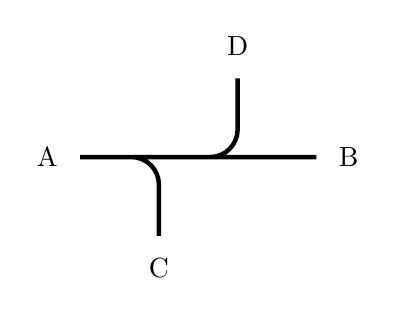
\begin{tikzpicture}
            \draw [rounded corners = 0.35cm, ultra thick]
            (0, 0) coordinate (A)
            (3,0) coordinate (B)
            (1,-1) coordinate (C)
            (2, 1) coordinate (D)
            (A) -- (B)
            (A) -- (A -| C) -- (C)
            (A) -- (A -| D) -- (D)

            (A) node [left = 4pt] {A}
            (B) node [right = 4pt] {B}
            (C) node [below = 4pt] {C}
            (D) node [above = 4pt] {D}
            ;
        \end{tikzpicture}
        &

        {\begin{minipage} [t] {0.4\linewidth}
            Connections:
            \begin{itemize}
                \setlength\itemsep{1pt}
                \item A, B, C, and D.
            \end{itemize}
        \end{minipage}
        \hfill
        \begin{minipage} [t] {0.4\linewidth}
            No connections:
            \begin{itemize}
                \setlength\itemsep{1pt}
                \item None.
            \end{itemize}
        \end{minipage}}

        \\ \midrule

        \begin{tikzpicture}
            \draw [ultra thick]
            (0, 0) coordinate (A)
            (3,0) coordinate (B)
            (1,-1) coordinate (C)
            (2, 1) coordinate (D)
            (A) -- (B)
            (A) -- (A -| C) -- (C)
            (A) -- (A -| D) -- (D)

            (A) node [left = 4pt] {A}
            (B) node [right = 4pt] {B}
            (C) node [below = 4pt] {C}
            (D) node [above = 4pt] {D}
            ;
        \end{tikzpicture}
        &

        {\begin{minipage} [t] {0.4\linewidth}
            Connections:
            \begin{itemize}
                \setlength\itemsep{1pt}
                \item A, B, C, and D.
            \end{itemize}
        \end{minipage}
        \hfill
        \begin{minipage} [t] {0.4\linewidth}
            No connections:
            \begin{itemize}
                \setlength\itemsep{1pt}
                \item None.
            \end{itemize}
        \end{minipage}}

        \\
        \bottomrule

    \end{xltabular}
\end{center}

\end{document}
